% !TEX program = xelatex
\documentclass[12pt,a4paper]{ctexart}
\usepackage{apacite}
\usepackage{xeCJK}
\usepackage{graphicx}
\usepackage{geometry}
\usepackage{lscape}



\begin{document}
    \title{消失的``红色地带'':意大利民主党支持者特征研究(2008-2018)\thanks{研究计划中使用的数据集和R代码可在https://github.com/zengchencn/ita-election-research-proposal 中获取。}}
    \author{曾宸\thanks{中国人民大学中共党史系2017级本科生,国际关系学院2021级研究生,本门课程为研究生先修课程。本科学号:2017202710。}}
    \maketitle

    \begin{abstract}
        意大利在战间期和战后有着西欧最强大的政治左翼力量,但在最近的2018年大选中,该国目前最大的中左翼政党——民主党的支持率下降明显,甚至在传统上被认为是意大利共产党和意大利左翼核心选区的中部``红色地带''也是如此。本研究计划使用意大利全国选举研究协会(ITANES)2008、2013、2018年大选的三次民调数据,通过Logistic模型来研究每次大选民主党支持者的群体特征,发现三次大选这些特征的变化。这篇研究计划通过对2018年大选调查的模型结果分析得出,民主党的支持者仍然将自己定位为左派和经济乐观主义者;他们来自小城镇,倾向于阅读《共和国报》,反对民粹主义。但是,这些支持者不再集中于意大利中部的``红色地带'',民主党选民的地理空间变化可能会导致意大利政治的不确定性,也为预测之后的大选结果带来了相当的不确定性。在正式的研究中,本文将2008、2013年的数据纳入讨论,并且将丰富数据来源、更好处理缺失值。
    \end{abstract}

    \textbf{关键词:} 民主党;意大利大选;投票行为;政党偏好

    \section{研究目的与研究意义}
    \subsection{研究缘起}
    在过去的一个世纪里,意大利拥有西欧最强大的政治左翼,在一定程度上使该国成为该地区政治最多元、博弈最激烈的地区之一。意大利共产党(\textit{Partito Comunista d'Italia}, PCd'I)成立于战间期,并逐渐成为二战期间意大利最大的反法西斯力量之一;其继承者意大利共产党(\textit{Partito Comunista Italiano}, PCI)仍然是战后意大利最大的反对党,并于长期处于执政地位的基督教民主党对峙,直至该党解体。
    \cite{gunther2000anchors}

    20世纪90年代初,意大利的政治格局发生了深刻的变化,共产党和基督教民主党相继解体;同南欧其他国家经过第三波民主化浪潮后的政治稳定相比,意大利政坛却充满了不确定因素。进入新世纪以来,新政党的形成和现代民粹主义的崛起产生了一种半稳定的三极平衡——中右翼联盟、反建制的五星运动和由民主党(\textit{Partito Democratico}, PD,成立于2007年)领导的中左翼联盟之间的平衡。
    \cite{pasquino2009democratic,fischer2012spatial}
    
    在2018年的大选中,选民对民主党及其领导的中左翼联盟的支持大幅度下降;民主党的支持者在全国各地急剧萎缩。这种趋势在意大利中部尤其明显,而这些地区以前常常被认为是有着共产主义同情者倾向的``红色地带''(\textit{Zona Rossa})。如图所示\ref{gen1318},红色区块代表中左翼联盟(主要是民主党)的选民,蓝色代表中右翼联盟,黄色代表五星运动。对比2013年大选的结果,2018年的结果显示,民主党的议席明显萎缩,北部的中右联盟和南部的五星运动接管了原来属于民主党和中左翼联盟的议会席位。


    \begin{figure}
        \centering
        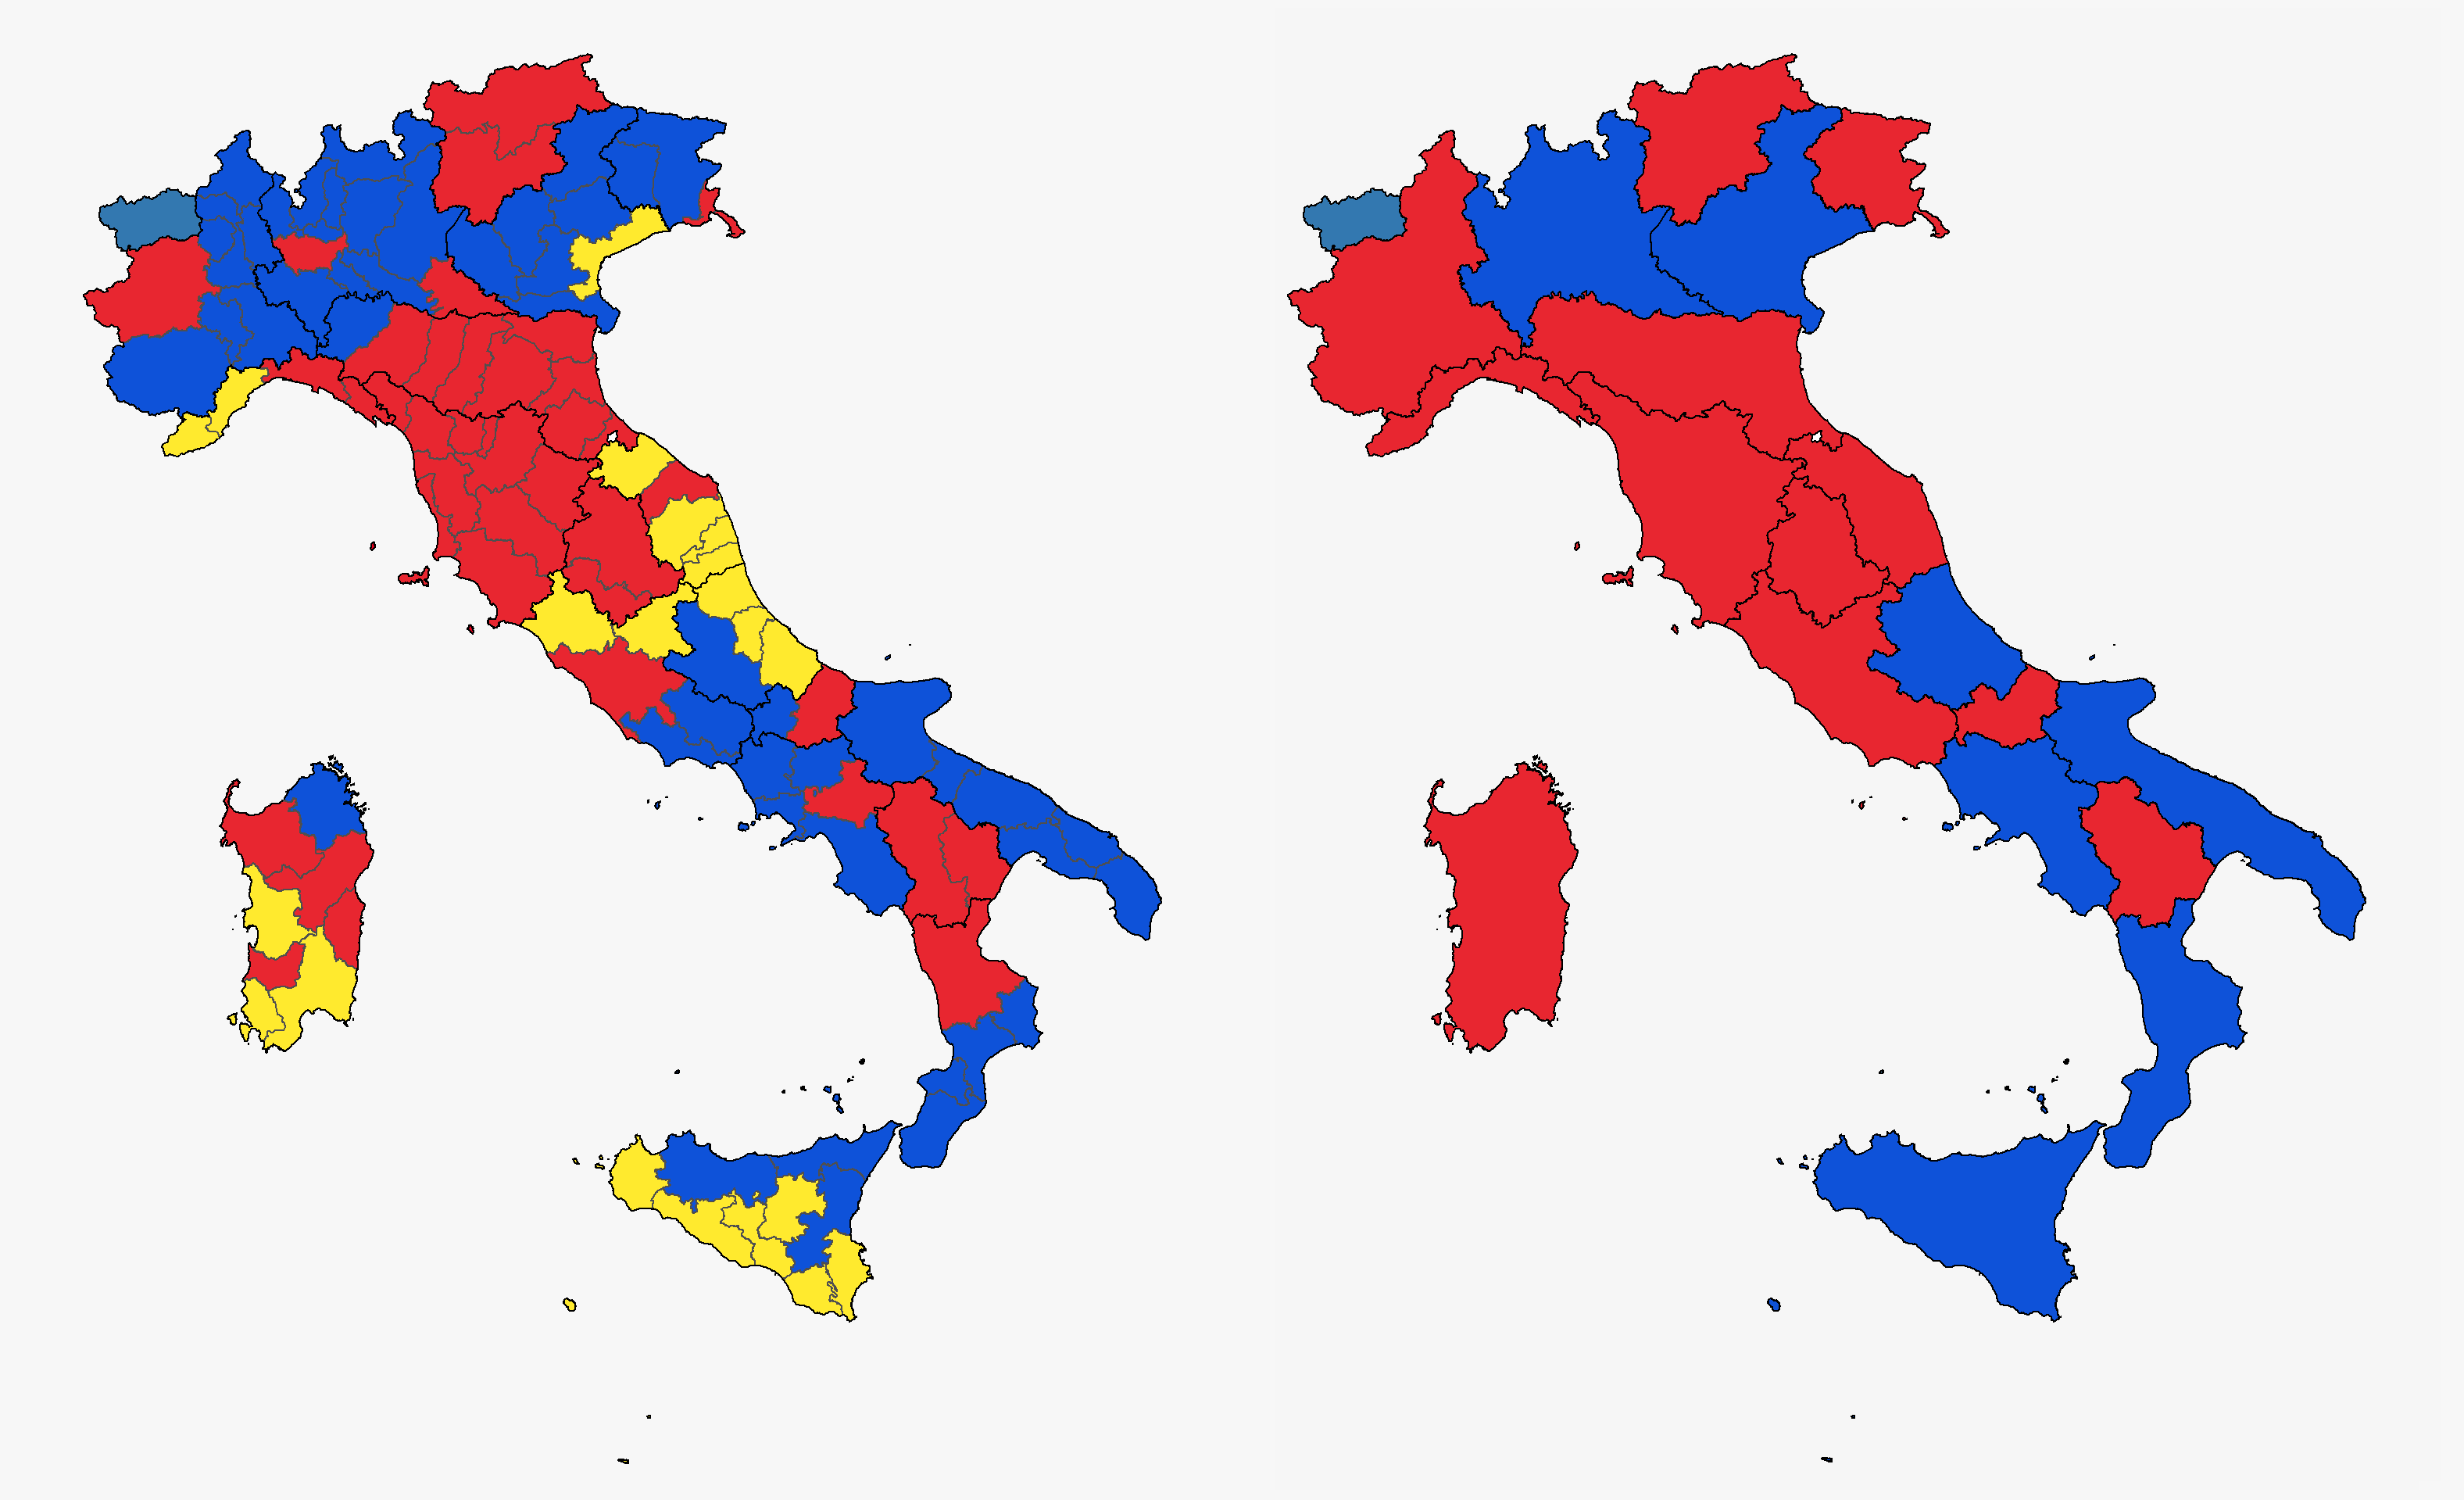
\includegraphics[width=0.6\textwidth]{images//2013gen.png}
        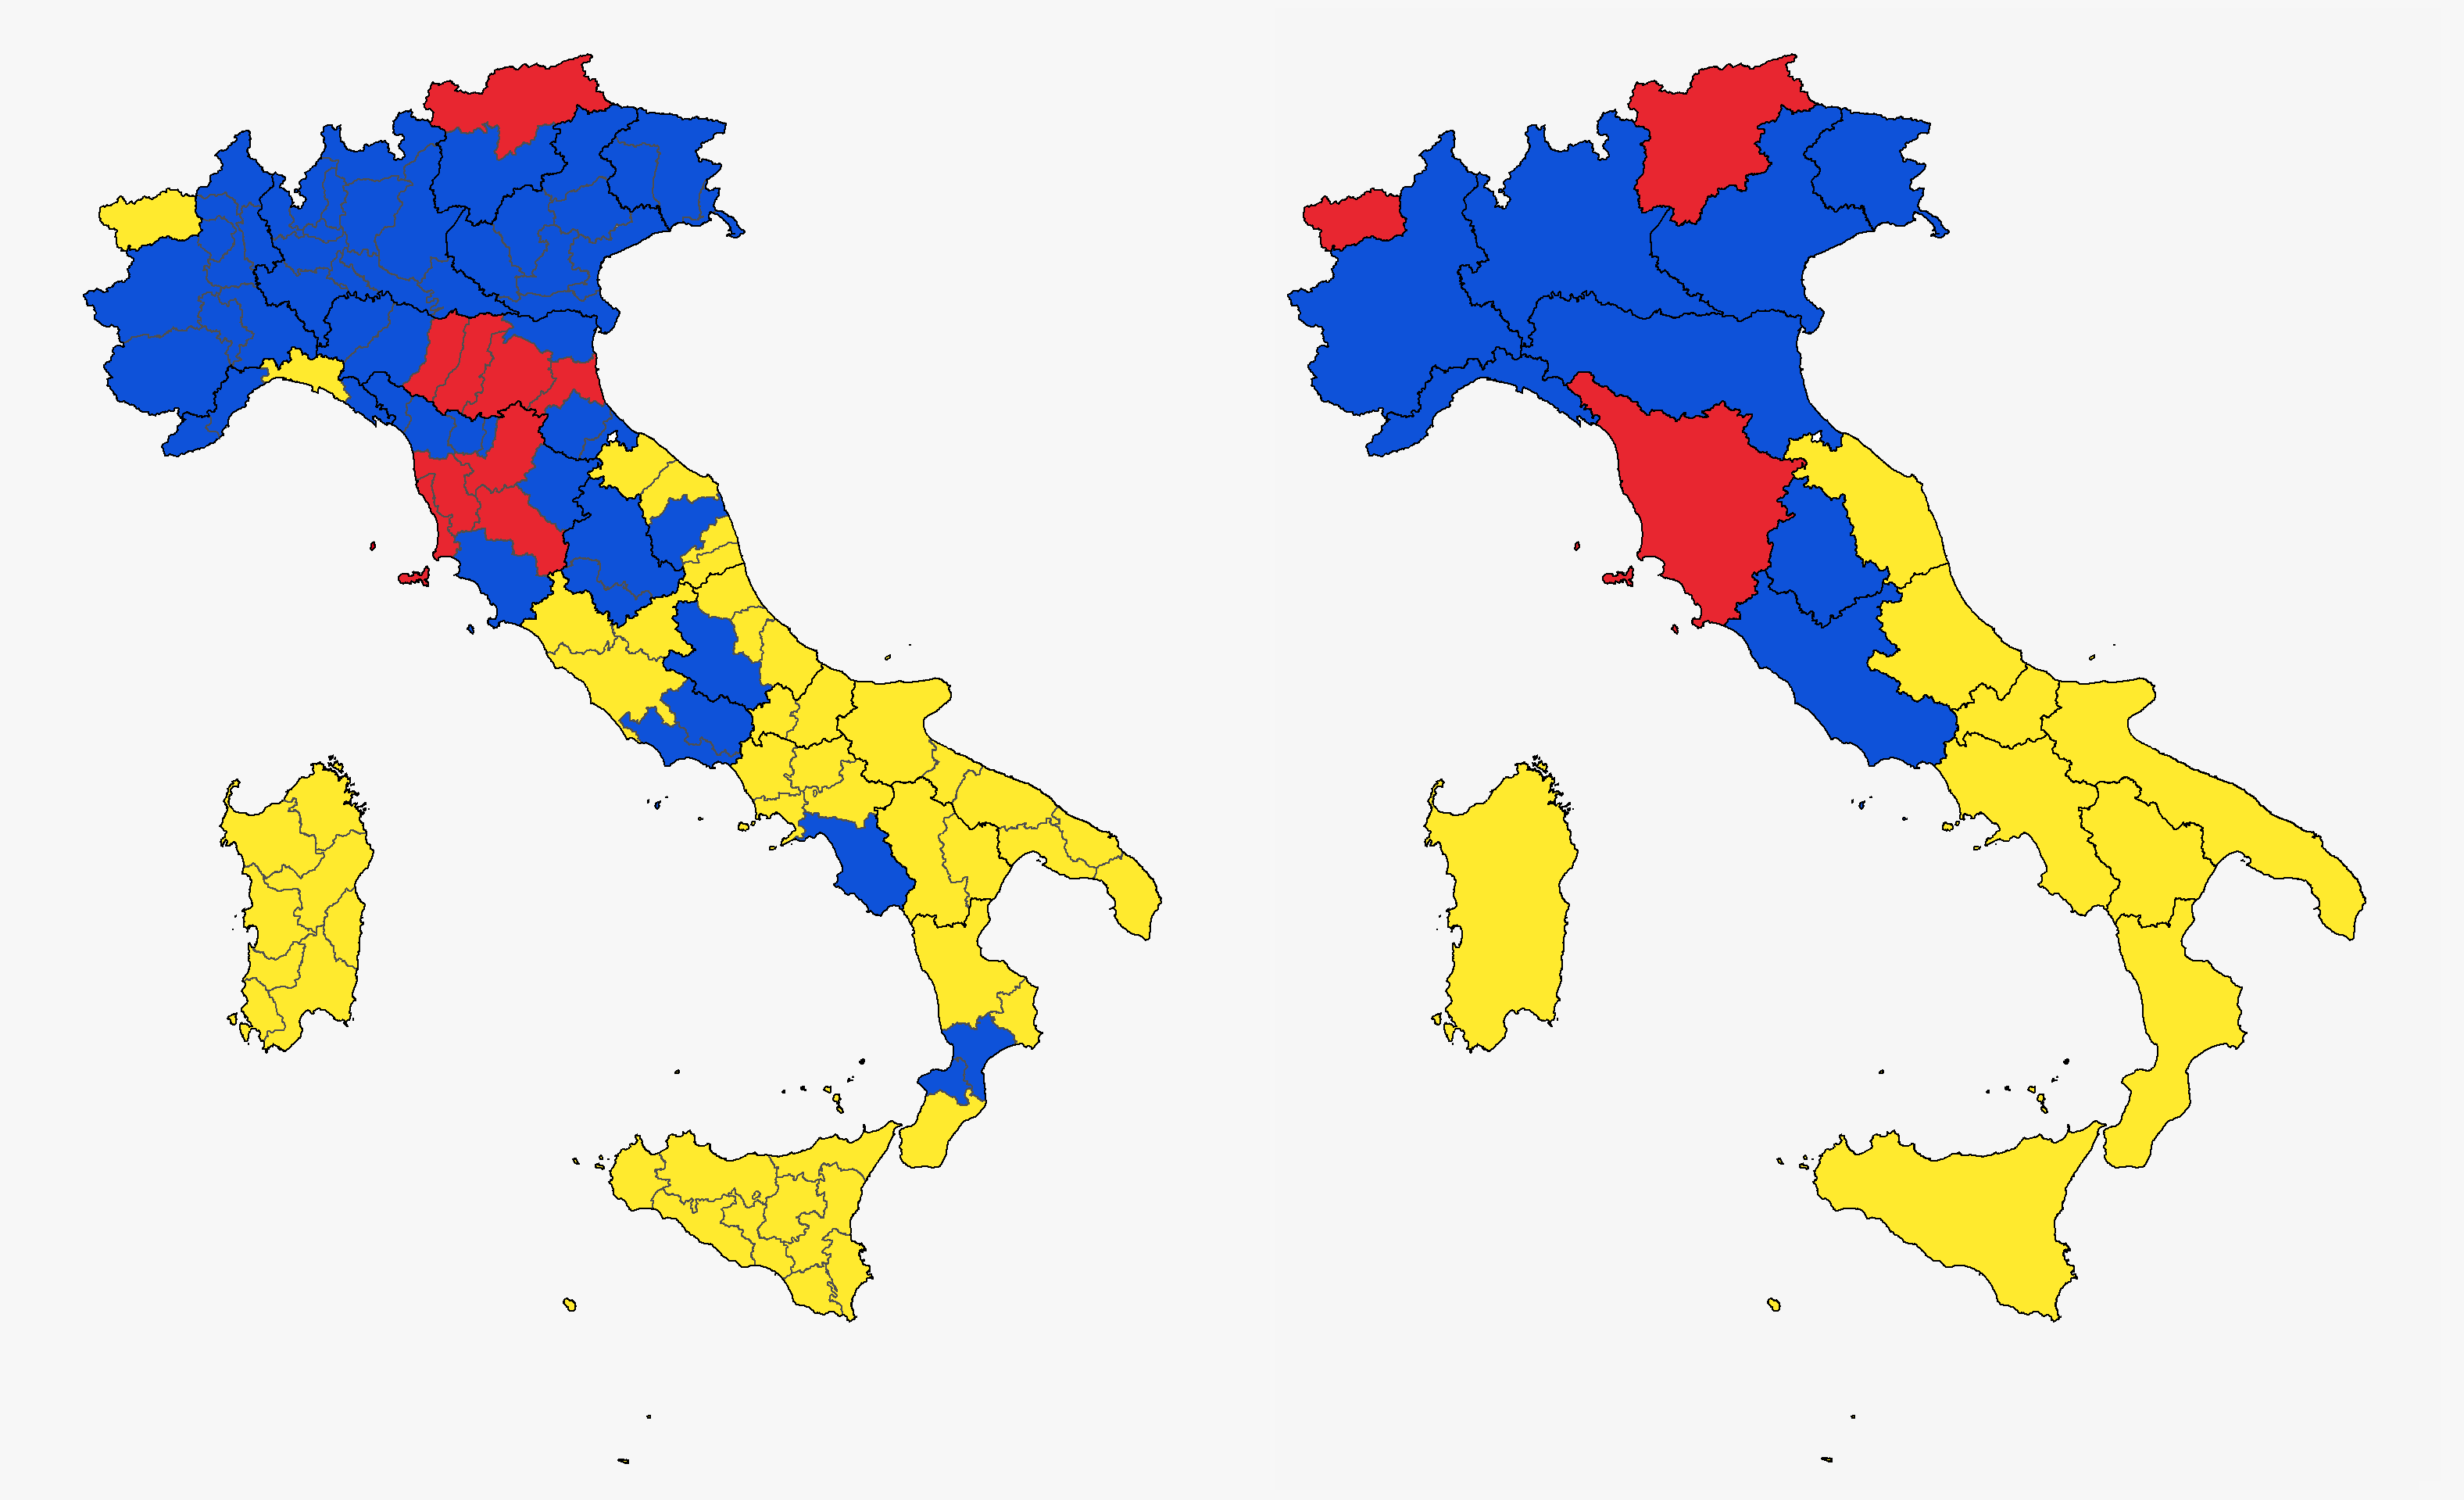
\includegraphics[width=0.6\textwidth]{images//2018gen.png}
        \caption{大选结果:2013 (上),2018 (下)}
        \label{gen1318}
    \end{figure}
    
    \subsection{研究目的与研究问题}
    笔者计划研究意大利民主党支持者的群体特征在2008、2013、2018年三次大选中的变化,探讨民主党支持者地理分布的变化和影响选民支持民主党的社会--经济因素。研究的主要问题包括:民主党的支持者是否倾向于将自己定位为政治左翼?民主党的支持者是否具有地理分布上的集中趋势?民主党的支持者是否倾向于阅读特定的报纸?民主党的支持者对民粹主义的看法如何?他们对意大利经济的发展和经济前景的看法如何?他们的这些群体特征在经历了三次大选之后,是否发生了变化?

    在这篇研究计划中,笔者将只对2018年的调查数据进行具体的建模分析;对最后一个问题的回答,将在正式的研究中展开。

    \subsection{研究意义}
    本研究具有一定的理论意义和现实意义。理论上,本研究以民主党的支持者群体特征为研究对象,描述意大利政党政治在过去十几年的变化,尤其是人口学特征的变化,讨论既有的``红色地带''等理论在2018年大选后为何已经变得过时。

    本研究还具有一定的现实意义,意大利政党政治的这一最新趋势意味着该国的政治平衡可能发生一些根本意义上变化,同时也意味着该国即将举行的大选变得更加难以预测。这种变化带来的不确定性可能会对意大利的对外关系,以及欧盟内部的政治格局产生影响,都需要引起利益相关者的重视。

    \section{文献综述与变量设定}

    在选举中对某一政党的强烈偏好传统上被归结为政党认同,这种在政治心理上的认同甚至可以与宗教热情相提并论。但是,这种美国式的政党认同的理论受到了欧洲地区选举研究的挑战,因为在欧洲,政党在政治舞台上占据了中心位置,而不是卡里斯玛型的政治家。
    \cite{berglund2005party}
    研究投票行为的传统方法强调了政党身份、现任者的表现、选民对选举间期社会经济发展的看法以及对候选人的看法这几个变量的重要性。
    \cite{fiorina1977outline}
    在许多欧洲国家,人们对某一政党而非个别政治家的忠诚度很高,因此,研究人员更关注非个人因素如何影响选民的政党偏好。

    具体到意大利的情况,研究者应该考虑到几个独特的因素——政治派别的区域分布、特定的媒体偏好以及与新近崛起的五星运动党有关的民粹主义意识形态。

    研究拟采用来自ITANES(意大利国家选举研究)协会的2008、2013和2018年选举后调查的数据集。\footnote{调查问卷和数据集可从http://www.itanes.org/获得。}在这篇研究计划中,笔者将以2018年的数据为例进行建模分析。如图\ref{num_survey}所示,为了更清晰地分析,本文将重点分析4个政党;在过滤缺失值后,这四个政党仍然拥有超过300个有效观测值。这一组政党都是当今意大利议会两院中最大的四个政党,它们涵盖了政治光谱的所有不同向度——中左翼的民主党、中右翼的联盟党和意大利力量党以及反建制的五星运动。

    \begin{figure}
        \centering
        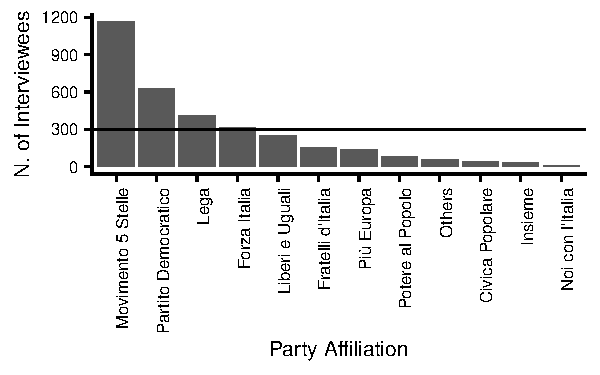
\includegraphics[width=1\textwidth]{figure//unnamed-chunk-2-1.pdf}
        \caption{受访者的政党偏好}
        \label{num_survey}
    \end{figure}

    研究重点关注五类变量——政治自我定位、人口特征、是否阅读《共和国报》(\textit{La Repubblica})、选民的民粹主义倾向和对经济前景的看法。以下各小节解释了选择这些变量的原因以及它们在调查结果中的体现。

    \subsection{政治自我定位}

    政治上的自我定位在预测选民的党派和支持特定政策的倾向方面是有效的,尽管有时需要考虑教育水平和这种自我定位的表达。
    \cite{coughlin1998grid,lesschaeve2017predictive}
    
    在ITANES收集的数据中,政治定位的回答以0--10为单位,0代表极左,10代表极右。图\ref{positioning}显示了四个政党在其支持者和所有受访者中的左右定位。这张图明显地体现了意大利政治中的左--右分化。无论是对于某个特定政党的支持者还是对于该调查中的所有受访者,意大利力量党和联盟党都被定位为右翼,而民主党被定位为左翼。值得注意的是,反建制的民粹主义政党五星运动被所有受访者定位在中间位置,而其支持者则更倾向于认为该党的意识形态为中间偏左。

    \begin{figure}
        \centering
        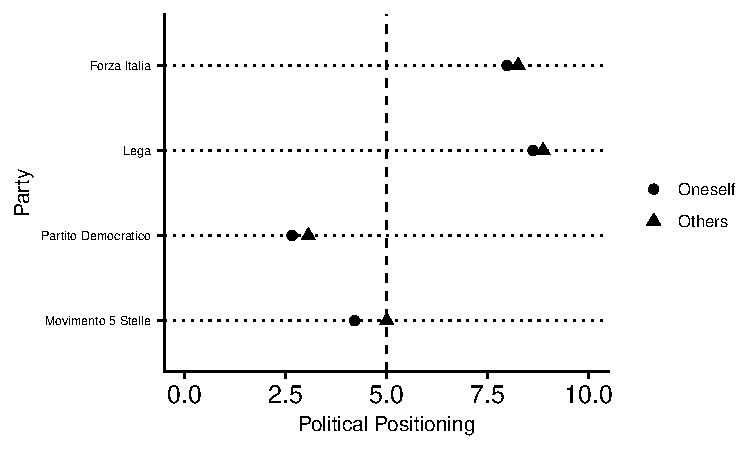
\includegraphics[width=1\textwidth]{figure//unnamed-chunk-3-1.pdf}
        \caption{政党的左右定位}
        \label{positioning}
    \end{figure}

    \subsection{人口学特征}

    意大利政治以其强烈的区域性特征而闻名。其中,意大利中部在历史上的反教会情绪和在20世纪对共产党的强烈支持,使该地区成为该国左翼政党的核心选区。这一趋势在小城镇和农村体现得尤为明显。这块区域常常被称为``红色地带''(\textit{La Zona Rossa})。
    \cite{shin2001whatever}
    ``红色地带''由四个大区组成——艾米利亚--罗马涅、托斯卡纳、翁布里亚和马尔凯,这些区域包含一些世界上最著名的城市,如佛罗伦萨和博洛尼亚。如图\ref{gen1318}所示,该区域在一直是民主党的核心选区;然而,在2018年的大选中,该区域对民主党的支持率基本下降了,``红色地带''明显缩小。

    \begin{figure}
        \centering
        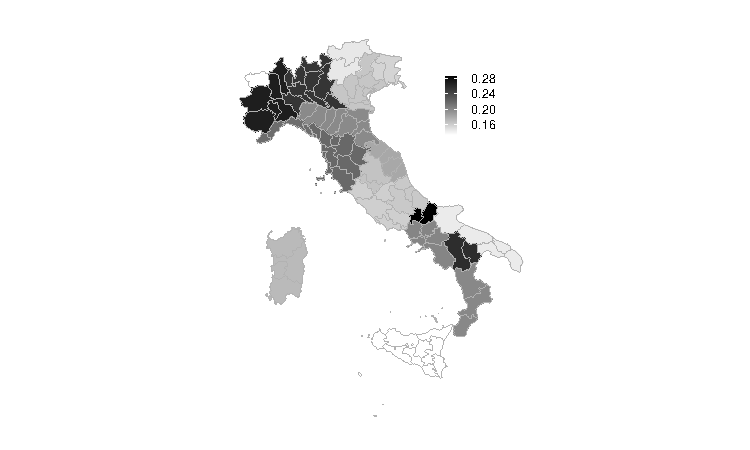
\includegraphics[width=1\textwidth]{figure//unnamed-chunk-4-1.pdf}
        \caption{民主党支持者在受访者中的比例}
        \label{pd_percent}
    \end{figure}

    图\ref{pd_percent}显示了在所有受访者中,明确表示支持民主党而非其他政党的受访者比例。支持民主党的比例最高的地区在西北部的皮埃蒙特大区和伦巴第大区,而不是传统意义上的红色地带。这可能意味着民主党支持者的地理分布可能发生了变化。本文将在后续章节中继续研究这一特征。

    此外,调查数据还包括了受访者居住的城镇大小,回答从1--4,居住的城镇人口数不断增大。

    \subsection{《共和国报》读者}

    政治极化的感知在很大程度上与媒体选择和媒体碎片化有关。
    \cite{davis2016party}
    在意大利,选民的媒体选择在很大程度上反映了他们的政治立场,因为一些媒体在报道政治人物和政治事件时常有自己的立场。在所有全国性的传播渠道中,《共和国报》(\textit{La Repubblica})是进步主义和政治左派的代表。
    \cite{tomasini2011anni}

    由于不同的媒体的总部和读者群常常分布在不同的城市(罗马、米兰和都灵),《共和国报》(\textit{La Repubblica})因其总部在罗马,政治倾向较为进步主义和同情左翼,其读者群与地理上的南北二分并不重合。如图\ref{rep_percent}所示,这部分读者的分布与图\ref{pd_percent}中可以看到的不同,应该单独设置变量对其进行考察。


    \begin{figure}
        \centering
        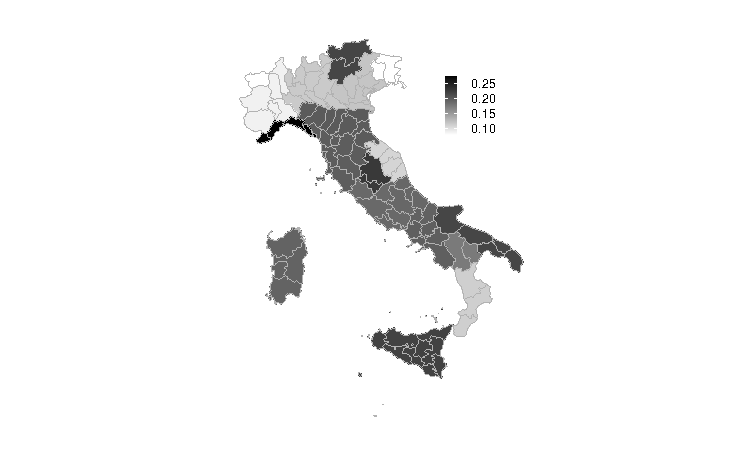
\includegraphics[width=1\textwidth]{figure//unnamed-chunk-5-1.pdf}
        \caption{受访者中每天阅读《共和国报》的比例}
        \label{rep_percent}
    \end{figure}


    \subsection{民粹主义倾向}

    本文设定的第5类变量是受访者对民粹主义意识形态的倾向。调查通过8个和民粹主义倾向相关的问题来考察受访者对民粹主义的不同方面的态度,这些问题分别是:

    \begin{enumerate}
        \item 议会中的政治人物必须遵循人民的意愿。 (\textit{I politici in Parlamento devono seguire la volontà dei cittadini})

        \item 应该由公民,而不是政治家来做出最重要的政治决定。 (\textit{I cittadini, e non i politici, dovrebbero prendere le decisioni politiche più importanti})

        \item 政治家和人民之间的差异比人民内部的差异更大。 (\textit{Le differenze fra i politici e il popolo sono maggiori delle differenze che ci sono all’interno del popolo})

        \item 我宁愿由一个普通人代表,而不是由一个专业的政治家代表。 (\textit{Preferirei essere rappresentato da una persona comune piuttosto che da un politico di professione})

        \item 政治家们说得多,做得少。 (\textit{I politici parlano tanto ma fanno poco})

        \item 在政治上做出妥协实际上意味着出卖自己的原则。 (\textit{Fare compromessi in politica significa in realtà svendere i propri principi})

        \item 记者过于关注和当权者的联系,而忽视和人民的联系。 (\textit{I giornalisti sono troppo a contatto con i poteri forti per informare le persone comuni})

        \item 国际大银行正在对我们的国家进行殖民。 (\textit{Le grandi banche internazionali stanno colonizzando il nostro Paese})
    \end{enumerate}

    受访者被要求在1--5的范围内给出答案,1表示强烈同意(\textit{Molto d'accordo}),5表示强烈不同意(\textit{Per niente d'accordo})。在随后的章节中,本文将分别考察对上述8个问题的每个回答。

    \subsection{经济发展展望}

    本文还考察受访者对经济发展与经济前景的态度,分析他们对经济发展的态度如何影响他们对民主党的支持。在采访中,受访者被要求对以下两个问题做出回答:

    \begin{enumerate}
        \item 让我们来谈谈经济问题。根据您的意见,意大利去年的经济形势...(\textit{Parliamo di economia. Secondo Lei la situazione economica in Italia nell'ultimo anno è...})

        \item 展望未来,您认为在未来12个月内,意大利的经济形势会... (\textit{Guardando ora al futuro, secondo Lei nei prossimi dodici mesi la situazione economica dell'Italia})
    \end{enumerate}

    受访者在1--5的范围内给出答案,1代表变好得多,5代表变差得多。

    \section{研究方法}

    研究旨在讨论促成选民对民主党的支持的因素。这是一个离散选择的问题,选民要么支持一个政党,要么不支持一个政党,只能有两种选择。\cite{fiorina1977outline,van2006rethinking}这种问题的实质说明要预测的因变量的结果是二分的,应该使用Logistic模型进行回归分析。本文根据上一节所讨论的变量设置,用Logistic模型来评估选民支持民主党的可能性。总共有16个变量——自我定位、地区(北部、中部、南部)、城镇规模、《共和国报》读者、民粹主义意识形态(8个问题)和经济前景(过去和未来)。

    研究的零假设是:选民支持民主党的可能性不受前面提到的16个变量的影响,我们在这里允许的I型错误率是0.05。

    \section{Logistic回归分析}

    表\ref{regression}显示了上一节所设定的模型的回归结果。此外,该表还补充了对其他政党或政党联盟的投票行为的分析——中左联盟、所有左派政党、中右翼的联盟党和意大利力量党,以及反建制的五星运动。

    \newpage
    \newgeometry{bottom=1cm}
    \begin{landscape}
        \begin{table}[!htbp] \centering 
    \caption{政党偏好的Logistic回归分析} 
    \label{regression} 
  \resizebox{1.6\textheight}{!}{%
  \begin{tabular}{@{\extracolsep{5pt}}lcccccc} 
  \\[-1.8ex]\hline 
  \hline \\[-1.8ex] 
   & \multicolumn{6}{c}{Party Choice} \\ 
  \cline{2-7} 
  \\[-1.8ex] & PD & Center-left & All Leftists & Lega & Forza & M5S \\ 
  \\[-1.8ex] & (1) & (2) & (3) & (4) & (5) & (6)\\ 
  \hline \\[-1.8ex] 
   Self-positioning & $-$0.248$^{***}$ (0.021) & $-$0.228$^{***}$ (0.018) & $-$0.451$^{***}$ (0.021) & 0.482$^{***}$ (0.031) & 0.399$^{***}$ (0.028) & $-$0.144$^{***}$ (0.016) \\ 
    Region - North & 0.434$^{***}$ (0.145) & 0.321$^{**}$ (0.136) & 0.403$^{***}$ (0.150) & 1.703$^{***}$ (0.215) & $-$0.212 (0.183) & $-$0.928$^{***}$ (0.140) \\ 
    Region - Center & $-$0.067 (0.165) & $-$0.022 (0.150) & 0.215 (0.160) & 1.672$^{***}$ (0.220) & $-$0.301 (0.193) & $-$0.786$^{***}$ (0.145) \\ 
    Region - South & $-$0.202 (0.159) & $-$0.172 (0.146) & $-$0.054 (0.156) & 1.251$^{***}$ (0.231) & $-$0.217 (0.194) & $-$0.391$^{***}$ (0.137) \\ 
    Town Size & $-$0.126$^{**}$ (0.049) & $-$0.112$^{**}$ (0.046) & $-$0.106$^{**}$ (0.049) & 0.010 (0.062) & $-$0.0004 (0.060) & 0.096$^{**}$ (0.046) \\ 
    La Rep. Reader & 0.434$^{***}$ (0.132) & 0.391$^{***}$ (0.128) & 0.935$^{***}$ (0.149) & $-$0.678$^{**}$ (0.313) & $-$0.132 (0.238) & $-$0.915$^{***}$ (0.154) \\ 
    Populism - General Will & $-$0.019 (0.074) & 0.087 (0.070) & 0.088 (0.080) & $-$0.278$^{**}$ (0.127) & $-$0.048 (0.105) & 0.160$^{**}$ (0.080) \\ 
    Populism - Direct Democracy & $-$0.094 (0.061) & $-$0.076 (0.057) & $-$0.051 (0.061) & $-$0.143$^{*}$ (0.084) & $-$0.005 (0.080) & 0.112$^{*}$ (0.059) \\ 
    Populism - People-politician Dispute & $-$0.057 (0.066) & $-$0.039 (0.062) & $-$0.049 (0.068) & 0.123 (0.093) & $-$0.042 (0.091) & 0.018 (0.066) \\ 
    Populism - Anti-professionalism & 0.335$^{***}$ (0.061) & 0.301$^{***}$ (0.057) & 0.449$^{***}$ (0.062) & 0.066 (0.079) & 0.073 (0.077) & $-$0.749$^{***}$ (0.063) \\ 
    Populism - Non-action Accusation & $-$0.021 (0.078) & $-$0.034 (0.074) & 0.006 (0.082) & $-$0.216$^{*}$ (0.119) & 0.232$^{**}$ (0.101) & $-$0.001 (0.085) \\ 
    Populism - Betraying Principles & 0.155$^{**}$ (0.061) & 0.167$^{***}$ (0.057) & 0.129$^{**}$ (0.063) & $-$0.045 (0.082) & 0.099 (0.079) & $-$0.061 (0.059) \\ 
    Populism - Journalist's Impact & 0.007 (0.067) & 0.033 (0.063) & 0.199$^{***}$ (0.071) & 0.119 (0.093) & 0.055 (0.089) & $-$0.256$^{***}$ (0.069) \\ 
    Populism - Intl Colonization & 0.177$^{***}$ (0.067) & 0.253$^{***}$ (0.064) & 0.128$^{*}$ (0.072) & $-$0.042 (0.094) & 0.016 (0.090) & 0.003 (0.069) \\ 
    Economic Overview - Past & $-$0.542$^{***}$ (0.086) & $-$0.515$^{***}$ (0.078) & $-$0.499$^{***}$ (0.083) & 0.227$^{**}$ (0.098) & $-$0.105 (0.094) & 0.278$^{***}$ (0.073) \\ 
    Economic Outlook - Future & $-$0.310$^{***}$ (0.090) & $-$0.286$^{***}$ (0.083) & $-$0.160$^{*}$ (0.088) & 0.008 (0.103) & $-$0.082 (0.100) & 0.038 (0.078) \\ 
    Constant & 1.173$^{***}$ (0.377) & 1.035$^{***}$ (0.348) & 1.518$^{***}$ (0.376) & $-$6.492$^{***}$ (0.550) & $-$4.603$^{***}$ (0.487) & 0.768$^{**}$ (0.342) \\ 
   \hline \\[-1.8ex] 
  Observations & 2,502 & 2,502 & 2,502 & 2,502 & 2,502 & 2,502 \\ 
  Log Likelihood & $-$1,013.578 & $-$1,150.508 & $-$1,009.527 & $-$647.242 & $-$719.762 & $-$1,177.450 \\ 
  Akaike Inf. Crit. & 2,061.155 & 2,335.016 & 2,053.054 & 1,328.484 & 1,473.524 & 2,388.900 \\ 
  \hline 
  \hline \\[-1.8ex] 
  \textit{Note:}  & \multicolumn{6}{r}{$^{*}$p$<$0.1; $^{**}$p$<$0.05; $^{***}$p$<$0.01} \\ 
  \end{tabular} 
  }
  \end{table} 
    \end{landscape}

    \newpage
    \restoregeometry

    对表\ref{regression}中的所有模型进行似然比检验(likelihood ratio test)的结果显示,对于所有6个模型,Pr(>Chisq)<0.001都成立,这说明这6个模型在设定的显著性水平(0.05)上是整体有效的,因此研究拒绝零假设,接受替代假设。

    回归结果显示,当一个人更趋向于将自己定位政治上的右派时,其投票给民主党的可能性就会大大降低;这种倾向也可以从其他左派政党和五星运动中观察到。中右翼政党的情况则相反。这验证了以往文献对这一问题认识的正确性,也符合对数据所作的探索性分析。

    分析意大利政治和政党偏好的区域特征,与之前文献综述中提到的红色区域相比,北部地区更倾向与支持民主党,但在这一倾向和其他地区没有显著相关性。其他左派政党也显示出相似的分布特征。联盟党,即以前的北方联盟(\textit{Lega Nord}),在北方的支持率也比其他地区都要强。

    受访者居住的城镇的大小也影响着对民主党的支持。在回归结果中,该变量的负系数表明,来自大城市的人投票给民主党的可能性就比来自小城镇或者农村的人来说要小。这一倾向在其他左翼政党中同样存在,它与农村地区、小城镇居民更加支持共产党及其后继者的传统观念相吻合。与此相反的是,受访者对五星运动的支持随着城镇规模的扩大而增加。

    在政治媒介方面,回归结果显示,阅读《共和国报》大大增加了投票给民主党和其他左派政党的可能性,同时大大降低了投票给联盟党或五星运动的可能性。然而,它对意大利力量党的投票影响并不显著。

    在民粹主义意识形态方面,民主党的支持者强烈反对业余政治家参政,反对政客们常常作出原则性妥协的指责,也并不认为意大利的主权正在受到损害。其他左翼政党也有类似的倾向;这与五星运动形成了鲜明的对比,五星运动对职业政治家有强烈的不满,认为政治这是临时的工作而非职业,同时认为外国势力正在危害意大利的国家主权。

    经济方面,民主党的支持者倾向于认为意大利的经济正在变好,而且对该国未来的经济发展感到乐观。联盟党和五星运动的支持者则对意大利未来一年的经济发展情况感到悲观。

    \section{进一步研究的空间}

    从2013年大选到2018年大选,在意大利中部,特别左翼势力强大的红色地带,民主党和政治左派的支持者大量减少。意大利左翼的传统刻板印象,即来自中部地区``红色地带''的小城镇居民,已经被2018年大选证明是部分错误,或者至少是解释力不够的。

    本文对2018年大选调查数据的分析否认了来自意大利中部地区的``红色地带''的人更加倾向于支持民主党的传统观念,事实上,来自北方地区的人更倾向于支持民主党和其他左翼政党。但是,来自小城镇的人倾向于支持民主党的这一特征没有改变。这一发现在一定程度上暗示了民主党支持者分布的地理变化,以及对该党的支持在全国范围内的减少;但此外,媒体选择和政党偏好之间的强关联性也可能为民主党寻找新的支持者开辟了一个新的战略途径。凡此种种,由``红色地带''缩小引发的意大利政治格局的变化可能只是意大利政治发展充满不确定的未来的前奏。

    在后续的研究中,笔者将使用相同的模型对2008年、2013年的调查数据进行分析,寻找在探索性描述中体现的差异是否在统计学上显著。在后续的研究中,笔者会根据实际情况加入年龄、受教育程度、政治参与积极性等变量(这些变量在2018年的模型中是不显著的),额外使用Eurobarometer等数据来源来对这一研究的背景进行补充。此外,在正式的研究中笔者还将更好地对数据集中的缺失值进行处理。

    \bibliographystyle{apacite}
    \bibliography{ref.bib}
\end{document}
